% Phần ALS và Cholesky. Người viết: Hồ Nguyễn Anh Tuấn.
% Số liệu đo trên MovieLens-1M (bộ dữ liệu chung của nhóm), baseline là BiasBaseline của nhóm.
% Mọi số chỉ dùng train và val; RMSE trên test nằm ở phần so sánh tổng.
% Preamble cần: amsmath, graphicx, float, array, tikz (thư viện arrows.meta, positioning); nếu biên dịch bằng XeLaTeX thì đặt \setmonofont
% bằng font có dấu tiếng Việt (ví dụ Consolas) để khối code hiển thị đúng chú thích.
\section{ALS và bộ giải Cholesky}

\subsection{Bài toán}

Bài toán của một hệ gợi ý phim rất đời thường: \emph{một người đã chấm điểm một số phim, vậy họ sẽ chấm
bao nhiêu điểm cho những phim chưa xem?} Nếu đoán được, ta chỉ việc gợi ý những phim có điểm dự đoán cao
nhất.

Dữ liệu là một bảng điểm $R$ cỡ $m \times n$: hàng $u$ là người dùng $u$, cột $i$ là phim $i$, ô $(u, i)$
chứa điểm $r_{ui}$. Phim nào người đó chưa xem thì ô bỏ trống, ký hiệu ``?'':
\[
  R = \begin{array}{r@{\quad}c}
    & \begin{array}{cccc} \text{phim } 1 & \text{phim } 2 & \cdots & \text{phim } n \end{array} \\[2pt]
    \begin{array}{r} \text{người } 1 \\ \text{người } 2 \\ \vdots \\ \text{người } m \end{array} &
    \left(\begin{array}{cccc} r_{11} & ? & \cdots & r_{1n} \\ ? & r_{22} & \cdots & ? \\
      \vdots & \vdots & \ddots & \vdots \\ r_{m1} & ? & \cdots & r_{mn} \end{array}\right)
  \end{array}
\]
MovieLens-1M có $6\,040$ người dùng và $3\,706$ phim, tức khoảng 22,4 triệu ô, nhưng tập train chỉ có
$800\,203$ điểm: \textbf{khoảng 96,4\% bảng đang trống}. Nhiệm vụ của ALS là điền các ô trống đó đủ chính
xác để chọn ra những phim người dùng có khả năng thích nhất.

\subsection{Ý tưởng: mỗi người và mỗi phim là một vector}

Ý tưởng chính là điểm số không ngẫu nhiên, mà do một vài \textbf{nhân tố ẩn} quyết định: một phim có bao
nhiêu phần hành động, bao nhiêu phần lãng mạn, là phim kinh điển hay phim thương mại; và một người thích
từng thứ đó đến mức nào.
\begin{itemize}
  \item Mỗi người $u$ có một vector $p_u \in \mathbb{R}^k$: ``hồ sơ gu'' của người đó với từng nhân tố.
  \item Mỗi phim $i$ có một vector $q_i \in \mathbb{R}^k$: ``hồ sơ đặc điểm'' của phim với từng nhân tố.
\end{itemize}
Điểm dự đoán là \textbf{tích vô hướng} của hai vector, tức nhân từng cặp rồi cộng lại:
\begin{equation}
  \hat r_{ui} = p_u^\top q_i = p_{u1} q_{i1} + p_{u2} q_{i2} + \dots + p_{uk} q_{ik} .
\end{equation}
Người thích hành động gặp phim nhiều hành động thì tích lớn, điểm cao; gu và phim lệch nhau thì tích âm,
điểm thấp. Các nhân tố không được đặt tên trước: mô hình tự học chúng từ bảng điểm, không dùng cột thể loại
phim. Số nhân tố $k$ là siêu tham số do ta chọn.

Xếp các $p_u$ thành hàng của ma trận $P$ (cỡ $m \times k$) và các $q_i$ thành hàng của $Q$ (cỡ
$n \times k$). Theo quy tắc nhân ma trận, ô $(u, i)$ của $PQ^\top$ đúng bằng $p_u^\top q_i$, nên cả bảng
dự đoán là tích của hai ma trận:
\[
  P = \begin{pmatrix} p_1^\top \\ p_2^\top \\ \vdots \\ p_m^\top \end{pmatrix},\qquad
  Q = \begin{pmatrix} q_1^\top \\ q_2^\top \\ \vdots \\ q_n^\top \end{pmatrix},\qquad
  \underbrace{R}_{m \times n} \approx \underbrace{P}_{m \times k}\, \underbrace{Q^\top}_{k \times n} .
\]
Nói cách khác, ALS \textbf{phân rã} một bảng khổng lồ và thưa thành hai ma trận nhỏ và đặc. Với
MovieLens-1M và $k = 20$, thay vì 22,4 triệu ô ta chỉ cần học $(6\,040 + 3\,706) \times 20 \approx 195$
nghìn số. Dấu ``$\approx$'' chỉ đòi hỏi trên các ô đã biết; ở ô trống, $PQ^\top$ vẫn cho ra một con số,
và đó chính là dự đoán.

\paragraph{Kết hợp với baseline của nhóm.} Trong code, điểm dự đoán đầy đủ là
\begin{equation}
  \hat r_{ui} = \underbrace{\mu + b_u + b_i}_{\text{baseline của nhóm}} + \; p_u^\top q_i .
\end{equation}
Phần baseline nằm trong \texttt{src/models/baseline.py}: $\mu = 3{,}58$ là điểm trung bình toàn tập, $b_u$
cho biết người dùng chấm dễ hay khó, $b_i$ cho biết phim được đánh giá cao hay thấp hơn mức chung. Baseline
chưa cá nhân hóa: nó gợi ý cho mọi người gần như cùng một danh sách phim ``được khen nhiều''. ALS phân rã
\emph{phần dư} $r'_{ui} = r_{ui} - \mu - b_u - b_i$, tức phần ``khẩu vị riêng'' mà baseline chưa giải
thích được.

\subsection{Hàm mục tiêu: thế nào là ``khớp tốt''}

ALS tìm $P$ và $Q$ để cực tiểu
\begin{equation}
  J(P, Q) = \sum_{(u,i)\ \text{đã có điểm}} \left(r'_{ui} - p_u^\top q_i\right)^2
          + \lambda\left(\sum_u \|p_u\|^2 + \sum_i \|q_i\|^2\right).
  \label{eq:als-objective}
\end{equation}
\begin{itemize}
  \item \textbf{Số hạng đầu là sai số:} tổng bình phương chênh lệch giữa điểm thật và điểm dự đoán, chỉ
        tính trên các ô đã biết.
  \item \textbf{Số hạng sau là phạt}, với hệ số $\lambda > 0$: giữ các vector không quá lớn, để mô hình
        không ``học thuộc'' những người chỉ chấm vài phim.
\end{itemize}
$J$ càng nhỏ thì mô hình càng khớp dữ liệu mà vẫn không quá phức tạp.

\subsection{Vì sao phải ``luân phiên''}

Cái khó là trong $J$, $P$ và $Q$ nhân với nhau, nên $J$ không lồi theo $(P, Q)$ và không có công thức
nghiệm. Nhưng nếu \textbf{giữ cố định một bên}, ví dụ giữ $Q$, thì $J$ chỉ còn là hàm bậc hai theo $P$:
một bài toán bình phương tối thiểu giải được chính xác. ALS tận dụng điều đó: giữ $Q$, giải $P$; rồi giữ
$P$, giải $Q$; và lặp lại. Đó là ý nghĩa của tên gọi \emph{Alternating Least Squares}, bình phương tối
thiểu luân phiên.

Mỗi lần giải cho nghiệm tốt nhất khi bên kia đứng yên, nên $J$ \textbf{không bao giờ tăng} qua các bước.

\subsection{Công thức của một bước}

\paragraph{Mỗi người dùng là một bài toán Ridge (Chương 3).}
Khi $Q$ cố định, các số hạng của từng người dùng trong $J$ tách rời nhau, nên có thể giải từng $p_u$
riêng. Gọi $Q_u$ là ma trận chỉ gồm các hàng $q_i$ của những phim $u$ đã chấm, $r_u$ là vector phần
dư tương ứng. Đặt đạo hàm theo $p_u$ bằng 0 được hệ phương trình chuẩn của hồi quy Ridge:
\begin{equation}
  \underbrace{\left(Q_u^\top Q_u + \lambda I\right)}_{A_u \in \mathbb{R}^{k\times k}} p_u
  = \underbrace{Q_u^\top r_u}_{b_u} .
  \label{eq:als-ridge}
\end{equation}
Nói cách khác, ALS biến một bài toán tối ưu không lồi thành hàng nghìn bài hồi quy nhỏ: ``dựa vào các phim
người này đã chấm, ước lượng gu của họ''. Ba điểm cần nhớ:
\begin{itemize}
  \item $A_u$ chỉ có cỡ $k \times k$ (với $k = 20$ là $20 \times 20$), nên mỗi hệ rất nhỏ.
  \item Có $m$ người thì giải $m$ hệ độc lập, nên chạy song song được.
  \item Bước giải $Q$ làm y hệt, chỉ đổi vai trò: ``dựa vào những người đã chấm phim này, ước lượng đặc
        điểm của phim''.
\end{itemize}

\paragraph{Giải hệ bằng Cholesky (Chương 2).}
Với $\lambda > 0$, $A_u$ đối xứng xác định dương nên phân rã được duy nhất thành $A_u = LL^\top$ với
$L$ tam giác dưới:
\begin{equation}
  l_{jj} = \sqrt{a_{jj} - \sum_{m<j} l_{jm}^2}, \qquad
  l_{ij} = \frac{1}{l_{jj}}\left(a_{ij} - \sum_{m<j} l_{im} l_{jm}\right) \quad (i > j).
\end{equation}
Sau đó giải $Ly = b_u$ bằng thế xuôi và $L^\top p_u = y$ bằng thế ngược.

\paragraph{Vì sao Cholesky mà không phải LU hay nghịch đảo.}
\begin{itemize}
  \item Cholesky chỉ tốn khoảng $k^3/3$ phép tính, bằng một nửa LU, vì tận dụng tính đối xứng.
  \item Không cần chọn trụ và ổn định về số khi ma trận xác định dương.
  \item Tính $A_u^{-1}$ rồi nhân với $b_u$ vừa tốn hơn vừa kém chính xác hơn hai lần thế.
  \item Nếu gặp trụ không dương, Cholesky phát hiện ngay rằng ma trận không xác định dương; bộ giải tự cài
        dùng điều này để báo lỗi khi $\lambda = 0$ thay vì trả về kết quả sai.
\end{itemize}

\subsection{Các bước giải}

\begin{figure}[H]
\centering
\begin{tikzpicture}[node distance=7mm and 10mm,
  box/.style={draw, rounded corners, align=center, minimum width=34mm, minimum height=10mm, fill=gray!8},
  arr/.style={-{Stealth[length=2.5mm]}, thick}]
  \node[box] (init) {Khởi tạo $Q$\\(ngẫu nhiên nhỏ)};
  \node[box, right=of init] (p) {Giữ $Q$, giải $p_u$\\cho từng người};
  \node[box, right=of p] (q) {Giữ $P$, giải $q_i$\\cho từng phim};
  \node[box, below=of q] (check) {$J$ hoặc RMSE val\\còn giảm đáng kể?};
  \node[box, below=of check] (out) {Dự đoán ô trống\\$\hat r_{ui} = \mu + b_u + b_i + p_u^\top q_i$};
  \draw[arr] (init) -- (p);
  \draw[arr] (p) -- (q);
  \draw[arr] (q) -- (check);
  \draw[arr] (check.west) -| node[pos=0.25, above] {có, lặp lại} (p.south);
  \draw[arr] (check) -- node[right] {không} (out);
\end{tikzpicture}
\caption{Vòng lặp ALS.}
\label{fig:als-loop}
\end{figure}

\begin{enumerate}
  \item Khởi tạo $Q$ bằng các số ngẫu nhiên nhỏ.
  \item Giữ $Q$, giải $p_u$ cho từng người bằng Cholesky.
  \item Giữ $P$, giải $q_i$ cho từng phim.
  \item Tính $J$ hoặc RMSE trên tập val; nếu còn giảm đáng kể thì quay lại bước 2.
  \item Khi dừng, dự đoán ô trống bằng $\hat r_{ui} = \mu + b_u + b_i + p_u^\top q_i$ rồi gợi ý các phim có
        điểm cao nhất.
\end{enumerate}

\subsection{Ví dụ minh họa}

Để dễ hình dung, xét 3 người chấm 4 phim, gồm hai phim hành động (HĐ1, HĐ2) và hai phim tình cảm (TC1, TC2).
Dấu ? là phim chưa xem:
\begin{table}[H]
  \centering
  \begin{tabular}{lcccc}
    \hline
         & HĐ1 & HĐ2 & TC1 & TC2 \\
    \hline
    An   & 5 & 4 & 2 & ? \\
    Bình & ? & 2 & 5 & 4 \\
    Chi  & 4 & ? & ? & 2 \\
    \hline
  \end{tabular}
  \caption{Bảng điểm của ví dụ minh họa.}
  \label{tab:als-toy}
\end{table}
\begin{enumerate}
  \item Trừ điểm trung bình $\mu = 28/8 = 3{,}5$ để được độ lệch: số dương là thích hơn mức trung bình.
        Ví dụ nhỏ chỉ trừ $\mu$ cho gọn; mô hình thật trừ cả $b_u$ và $b_i$.
  \item Chọn $k = 2$ nhân tố (tạm gọi là hành động và tình cảm), $\lambda = 0{,}5$, rồi chạy ALS. Mỗi bước
        giải các hệ $2 \times 2$ bằng Cholesky.
  \item $J$ giảm từ $13{,}91$ xuống $4{,}88$ chỉ sau vòng đầu, rồi đứng yên quanh $4{,}66$ từ khoảng
        vòng 10.
  \item Sau khi học, $P$ cho thấy An và Chi thích hành động, Bình thích tình cảm. Cộng lại $\mu$ để có điểm
        dự đoán cho các ô trống (Bảng~\ref{tab:als-toy-pred}).
\end{enumerate}
\begin{table}[H]
  \centering
  \begin{tabular}{lcc}
    \hline
    Ô trống & Dự đoán & Gợi ý? \\
    \hline
    An -- TC2   & 2,56 sao & không \\
    Bình -- HĐ1 & 2,46 sao & không \\
    Chi -- HĐ2  & 3,51 sao & có \\
    Chi -- TC1  & 2,93 sao & không \\
    \hline
  \end{tabular}
  \caption{Dự đoán cho các ô trống sau 30 vòng ALS.}
  \label{tab:als-toy-pred}
\end{table}
Chi được gợi ý HĐ2 vì Chi chấm điểm giống An, mà An thích HĐ2. Đây chính là tinh thần của \textbf{lọc cộng
tác}: học từ những người có gu giống mình.

\subsection{Ý nghĩa và lý do chọn ALS}

\paragraph{Học ``lý do'' chứ không ghi nhớ từng ô.} Mỗi người chỉ cần $k$ con số, nhờ vậy mô hình đoán được
cả những ô chưa có dữ liệu.

\paragraph{So với SVD cổ điển (Chương 4).}
SVD cho xấp xỉ hạng thấp tốt nhất (định lý Eckart--Young) nhưng chỉ áp dụng cho ma trận \emph{đầy đủ}.
Muốn dùng SVD, ta phải điền 96,4\% ô trống bằng một giá trị giả định, thường là 0 hoặc trung bình, và
mô hình sẽ học cả những giá trị giả đó. ALS chỉ tính tổng trên các ô đã có điểm, nên không cần đoán
trước dữ liệu bị thiếu.

\paragraph{So với SGD (Chương 5).}
SGD đi từng bước nhỏ theo gradient và cần chọn learning rate: quá lớn thì phân kỳ, quá nhỏ thì chậm.
ALS ở mỗi bước tìm \emph{nghiệm đúng} của bài toán con, nên:
\begin{itemize}
  \item hàm mục tiêu $J$ không bao giờ tăng (đã kiểm chứng bằng test và trên dữ liệu thật);
  \item không có learning rate, chỉ có hai tham số $k$ và $\lambda$;
  \item hội tụ sau ít vòng: trên ML-1M, 5 vòng đầu đã đạt phần lớn mức cải thiện.
\end{itemize}

\paragraph{Song song hóa tự nhiên.}
Trong một bước, hệ của người dùng này không phụ thuộc hệ của người dùng khác. Do đó $9\,746$ hệ mỗi
vòng có thể giải đồng thời trên mọi lõi CPU, và kết quả không phụ thuộc số luồng. Đây cũng là lý do
ALS được dùng trong các hệ thống gợi ý quy mô lớn chạy phân tán, chẳng hạn thư viện MLlib của Spark.

\paragraph{Hạn chế.} Người mới có ít đánh giá vẫn được dự đoán kém tin cậy; $k$ và $\lambda$ phải dò trên
tập val.

\subsection{Áp dụng vào MovieLens-1M}

\subsubsection{Quy trình}

\begin{enumerate}
  \item \textbf{Baseline.} Fit \texttt{BiasBaseline} của nhóm trên tập train, rồi tính ma trận phần
        dư $R'$ ở dạng CSR. $R'$ có cùng các ô khác 0 như $R$.
  \item \textbf{Chuẩn bị hai chiều.} Giữ $R'$ (mỗi hàng là một người dùng) và chuyển vị $R'^\top$,
        cũng ở dạng CSR (mỗi hàng là một phim). CSR cho phép lấy các phim người dùng đã chấm trong
        thời gian tỉ lệ với số điểm của người đó (Chương 2).
  \item \textbf{Vòng lặp ALS.} Mỗi vòng giải $6\,040$ hệ để cập nhật $P$, rồi $3\,706$ hệ để cập
        nhật $Q$; cùng một hàm giải được dùng cho cả hai chiều.
  \item \textbf{Đánh giá và gợi ý.} Sau mỗi vòng ghi RMSE train, RMSE val, giá trị $J$ và thời gian.
        Khi gợi ý, dự đoán điểm cho mọi phim chưa xem, bỏ phim đã xem và lấy $N$ phim điểm cao nhất.
\end{enumerate}
Tham số dùng trong báo cáo: $k = 20$, $\lambda = 10$, 20 vòng. Đây là giá trị khởi đầu, chưa tinh
chỉnh trên tập val.

\subsubsection{Ví dụ tính tay: ước lượng gu của một người xem}

Để thấy một bước ALS làm gì, xét $k = 2$ với hai nhân tố đặt tên là ``hành động'' và ``tình cảm''.
Một người đã chấm ba phim; phần dư sau baseline và vector của ba phim (đang cố định) là:
\begin{center}
\begin{tabular}{lcc}
  \hline
  Phim & $q_i$ (hành động, tình cảm) & Phần dư $r'_{ui}$ \\
  \hline
  Phim hành động 1 & $(1{,}0;\ 0{,}2)$ & $+1{,}0$ \\
  Phim hành động 2 & $(0{,}8;\ 0{,}4)$ & $+0{,}8$ \\
  Phim tình cảm    & $(-0{,}5;\ 1{,}0)$ & $-0{,}6$ \\
  \hline
\end{tabular}
\end{center}
Người này chấm hai phim hành động cao hơn baseline dự đoán, và chấm phim tình cảm thấp hơn. Với
$\lambda = 0{,}1$, hệ~\eqref{eq:als-ridge} là
\[
  A = Q_u^\top Q_u + \lambda I = \begin{pmatrix} 1{,}99 & 0{,}02 \\ 0{,}02 & 1{,}30 \end{pmatrix},
  \qquad
  b = Q_u^\top r_u = \begin{pmatrix} 1{,}94 \\ -0{,}08 \end{pmatrix}.
\]
Cholesky cho $l_{11} = \sqrt{1{,}99} = 1{,}4107$, $l_{21} = 0{,}02/1{,}4107 = 0{,}0142$,
$l_{22} = \sqrt{1{,}30 - 0{,}0142^2} = 1{,}1401$. Thế xuôi $Ly = b$ được $y = (1{,}3752;\ -0{,}0873)$,
thế ngược $L^\top p = y$ được
\[
  p_u = (0{,}976;\ -0{,}077).
\]
Kết quả có ý nghĩa trực quan: người này \textbf{thích hành động} (hệ số dương lớn) và \textbf{hơi không
thích tình cảm}. Từ $p_u$, mô hình tái tạo phần dư của ba phim đã chấm là $0{,}96$; $0{,}75$; $-0{,}56$,
gần với giá trị thật nhưng nhỏ hơn một chút, do $\lambda$ kéo nghiệm về 0. Với một phim hành động
\emph{chưa xem} có $q = (0{,}9;\ 0{,}1)$, mô hình cộng thêm $p_u^\top q = +0{,}87$ điểm vào baseline;
với một phim tình cảm có $q = (-0{,}6;\ 0{,}9)$, mô hình trừ $0{,}65$ điểm. Kết quả của bộ giải tự cài
khớp với \texttt{numpy.linalg.solve}.

Trên dữ liệu thật, các nhân tố không có tên sẵn như ``hành động'' hay ``tình cảm''; mô hình tự tìm ra
chúng từ dữ liệu. Nhưng cơ chế tính hoàn toàn giống ví dụ trên, chỉ với $k = 20$ và hàng nghìn hệ.

\subsubsection{Vai trò của $\lambda$ dưới góc độ số (Chương 1 và 3)}

Sau khi chia tập, ML-1M có 401 người dùng có dưới 20 điểm trong train (ít nhất là 10). Với $k = 20$,
$Q_u^\top Q_u$ của những người này có hạng nhỏ hơn 20, tức suy biến: không có $\lambda$ thì hệ không có
nghiệm duy nhất. Với $\sigma$ là giá trị kỳ dị của $Q_u$, số điều kiện của hệ là
\begin{equation}
  \kappa_2\left(Q_u^\top Q_u + \lambda I\right) = \frac{\sigma_{\max}^2 + \lambda}{\sigma_{\min}^2 + \lambda}.
\end{equation}
Theo Chương 1, giải hệ có số điều kiện $\kappa$ mất khoảng $\log_{10}\kappa$ chữ số đáng tin.
Bảng~\ref{tab:als-kappa} đo $\kappa_2$ trên 200 người dùng lấy mẫu, dùng $Q$ đã học.

\begin{table}[H]
  \centering
  \caption{Số điều kiện theo $\lambda$ trên 200 người dùng lấy mẫu, MovieLens-1M, $k = 20$.}
  \label{tab:als-kappa}
  \begin{tabular}{rrrr}
    \hline
    $\lambda$ & $\kappa_2$ trung vị & $\kappa_2$ lớn nhất & Chữ số mất tối đa \\
    \hline
    0{,}01 & 13{,}3 & 2\,476 & 3{,}4 \\
    0{,}1 & 13{,}1 & 248{,}5 & 2{,}4 \\
    1 & 10{,}9 & 39{,}3 & 1{,}6 \\
    10 & 4{,}1 & 6{,}2 & 0{,}8 \\
    100 & 1{,}5 & 2{,}1 & 0{,}3 \\
    \hline
  \end{tabular}
\end{table}

\begin{figure}[H]
  \centering
  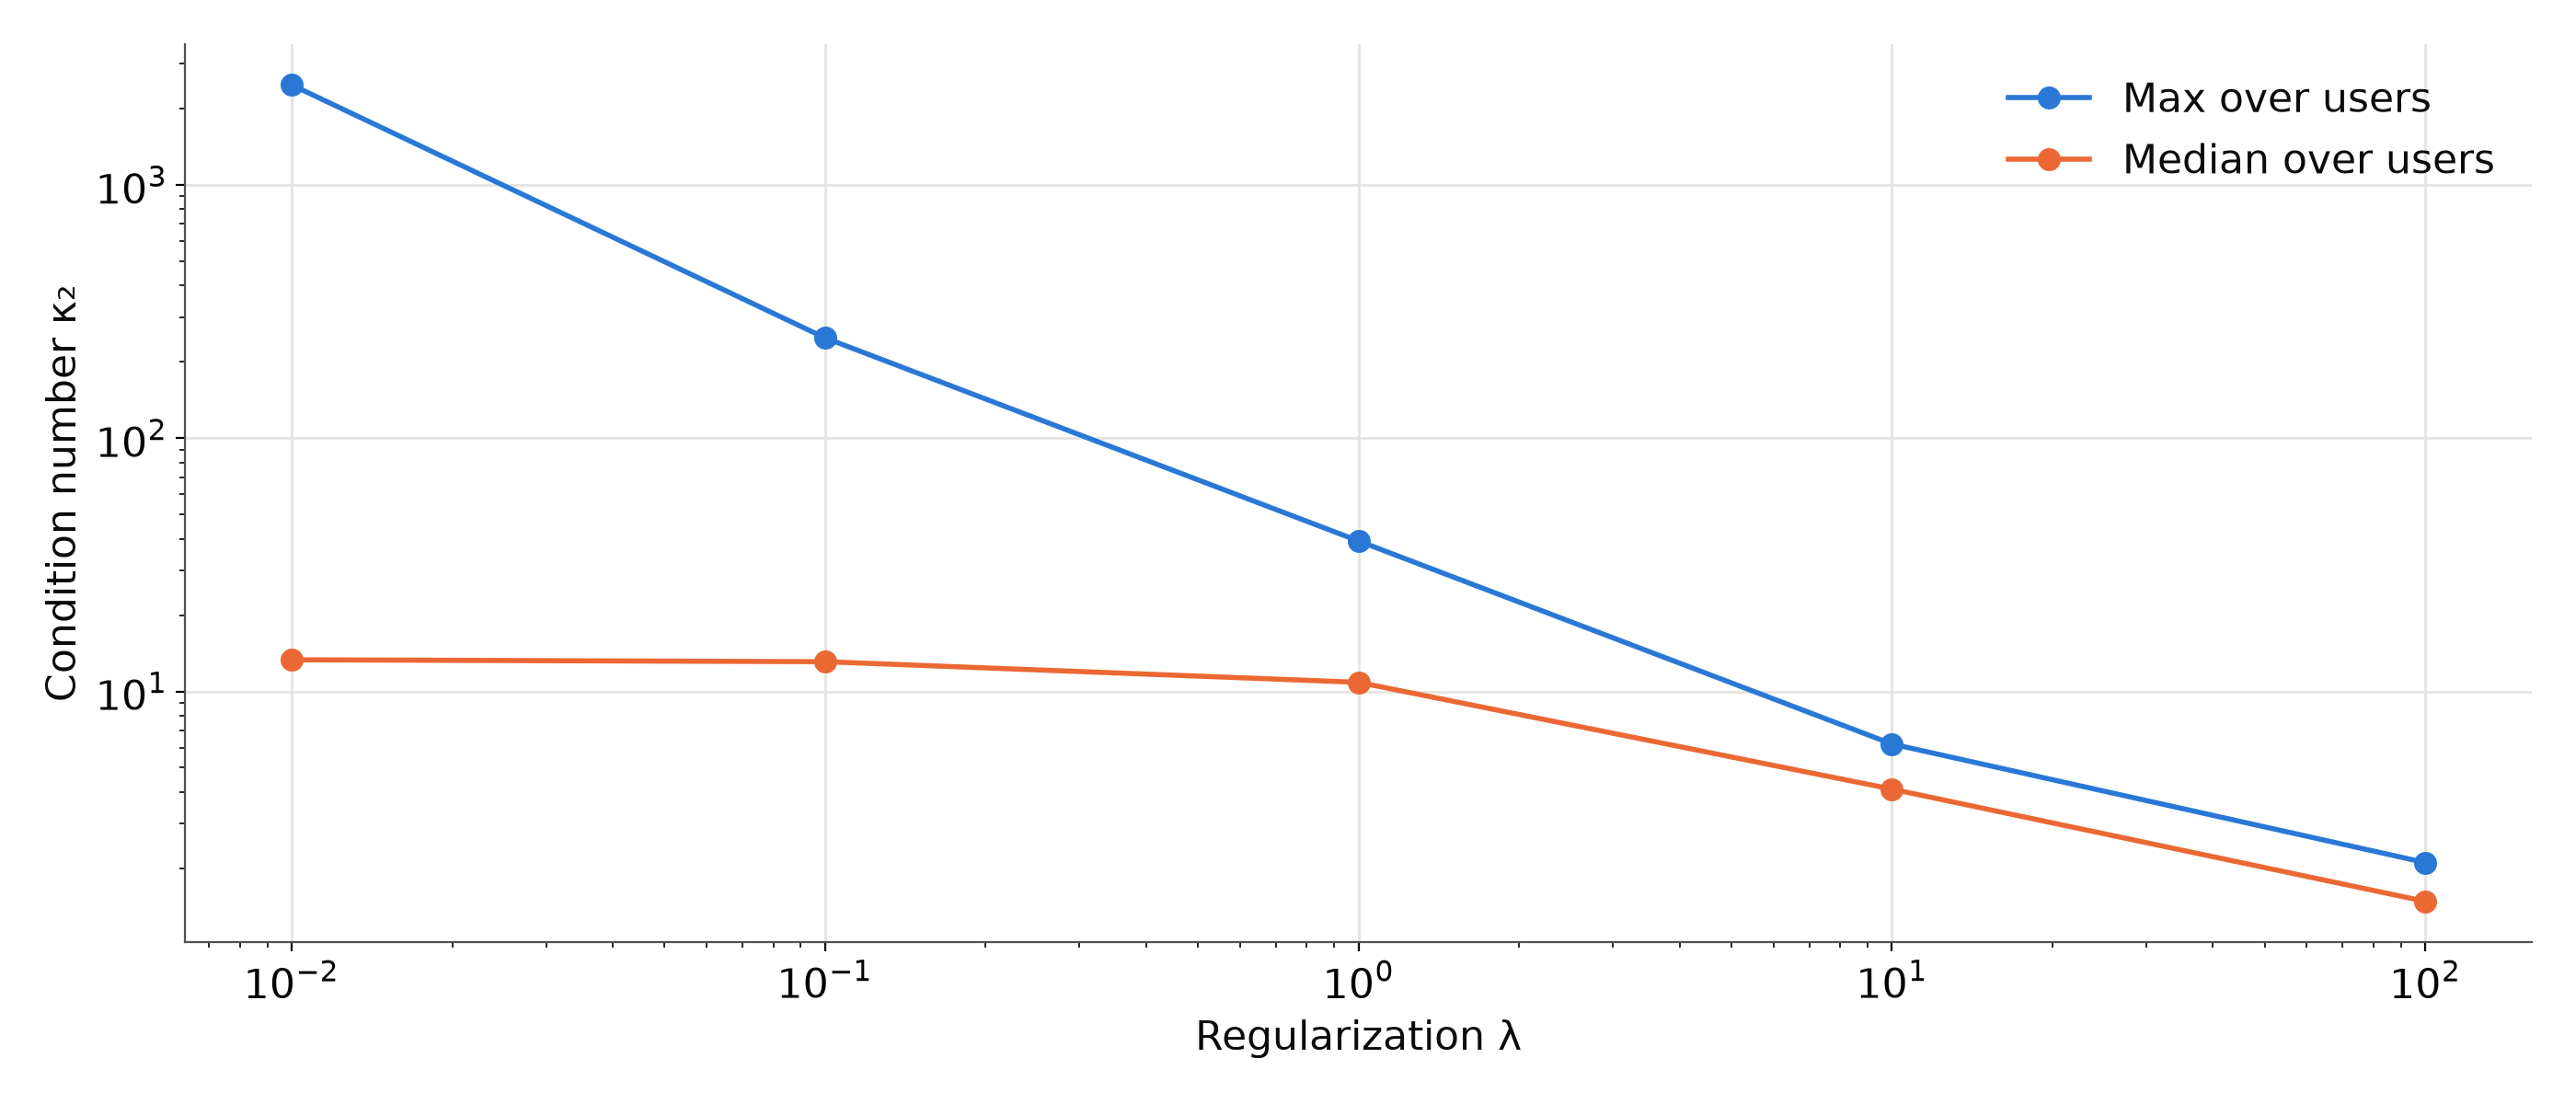
\includegraphics[width=0.85\linewidth]{figures/als_condition_vs_lambda.png}
  \caption{Số điều kiện theo $\lambda$, hai trục log.}
  \label{fig:als-kappa}
\end{figure}

Có hai điểm đáng chú ý. Thứ nhất, khi $\lambda$ giảm, trung vị gần như không đổi nhưng giá trị lớn nhất
tăng gần tỉ lệ với $1/\lambda$: với đa số người dùng, $\sigma_{\min}^2$ đã lớn hơn nhiều so với $\lambda$,
còn với người ít dữ liệu thì $\sigma_{\min} \approx 0$ và chỉ $\lambda$ giữ cho hệ ổn định. Thứ hai, $\lambda$
đóng hai vai trò cùng lúc: về thống kê, nó chống học thuộc; về số học, nó giữ $\kappa$ nhỏ. Với
$\lambda = 10$, hệ mất chưa tới 1 chữ số đáng tin trên khoảng 16 chữ số của float64.

\subsection{Cài đặt}

\subsubsection{Tổ chức code}

\begin{table}[H]
  \centering
  \caption{Các file thuộc phần ALS.}
  \label{tab:als-files}
  \begin{tabular}{p{0.36\linewidth}>{\raggedright\arraybackslash}p{0.56\linewidth}}
    \hline
    File & Vai trò \\
    \hline
    \texttt{src/solvers/linear.py} & Cholesky, thế xuôi, thế ngược tự cài; không dùng \texttt{numpy.linalg} \\
    \texttt{src/models/als.py} & Dựng và giải các hệ Ridge song song, hàm mục tiêu, lớp \texttt{ALSRecommender} \\
    \texttt{experiments/run\_als.py} & Đọc cấu hình, huấn luyện, ghi bảng hội tụ, đo số điều kiện, vẽ hình \\
    \texttt{tests/test\_models\_small.py} & Kiểm thử Cholesky và ALS trên ma trận nhỏ biết trước đáp án \\
    \hline
  \end{tabular}
\end{table}

\texttt{ALSRecommender} kế thừa lớp \texttt{Recommender} chung của nhóm và chỉ cài hai hàm
\texttt{\_fit} và \texttt{predict\_raw}. Việc giới hạn điểm trong khoảng 1--5, bỏ phim đã xem khi gợi ý
và lưu mô hình nằm ở lớp cha, nên ALS, SVD và SGD được đánh giá theo cùng một cách.

\subsubsection{Bộ giải Cholesky}

Hàm lõi ghi đè $L$ lên tam giác dưới của $A$ để không phải cấp phát ma trận mới, vì hàm này chạy
gần $10\,000$ lần mỗi vòng. Hàm trả về \texttt{False} thay vì ném lỗi, vì mã chạy song song trong numba
không ném lỗi được.
\begin{verbatim}
@njit
def _cholesky_core(A):
    k = A.shape[0]
    for j in range(k):
        pivot = A[j, j]
        for m in range(j):
            pivot -= A[j, m] * A[j, m]
        if not pivot > 0.0:          # bắt cả trụ âm lẫn NaN
            return False
        l_jj = np.sqrt(pivot)
        A[j, j] = l_jj
        for i in range(j + 1, k):
            value = A[i, j]
            for m in range(j):
                value -= A[i, m] * A[j, m]
            A[i, j] = value / l_jj
    return True
\end{verbatim}

\subsubsection{Dựng và giải các hệ song song}

Hàm \texttt{\_solve\_rows} nhận ma trận phần dư CSR và ma trận đang cố định. Mỗi hàng CSR là một hệ.
Vòng lặp ngoài dùng \texttt{prange} của numba nên các hệ chạy trên mọi lõi CPU. Chỉ tam giác dưới của
$A$ được dựng, vì Cholesky chỉ đọc phần đó, nhờ vậy bớt một nửa phép tính ở bước tốn kém nhất.
\begin{verbatim}
for row in prange(n_rows):                   # mỗi user (hoặc phim) một hệ
    A = np.zeros((k, k))
    x = solution[row]
    for pos in range(indptr[row], indptr[row + 1]):
        factor = fixed[indices[pos]]         # q_i của phim đã chấm
        value = data[pos]                    # phần dư r'_ui
        for a in range(k):
            x[a] += value * factor[a]        # b = Q_u^T r_u
            for c in range(a + 1):
                A[a, c] += factor[a] * factor[c]   # A = Q_u^T Q_u
    for a in range(k):
        A[a, a] += reg                       # + lambda I
    if _cholesky_core(A):
        _forward_core(A, x)                  # L y = b
        _backward_transpose_core(A, x)       # L^T p = y
    else:
        failed[row] = True
\end{verbatim}
Khi cập nhật $Q$, chỉ cần truyền ma trận chuyển vị (cũng ở dạng CSR) vào cùng hàm này. Vòng huấn
luyện vì thế rất ngắn:
\begin{verbatim}
for epoch in range(1, n_epochs + 1):
    P = update_factors(Q, residual, reg)          # cố định Q, giải P
    Q = update_factors(P, residual_by_item, reg)  # cố định P, giải Q
    log.record(epoch, elapsed, train_rmse, val_rmse, objective(P, Q, residual, reg))
\end{verbatim}

\subsubsection{Một số quyết định khi cài đặt}

\begin{itemize}
  \item \textbf{Đo thời gian đúng.} Numba biên dịch hàm ở lần gọi đầu. Trên ML-1M, bước này lâu gấp
        khoảng 40 lần một vòng ALS. Code gọi trước một hệ $1 \times 1$ để biên dịch xong rồi mới bắt đầu
        tính giờ, để so sánh thời gian với SGD được công bằng.
  \item \textbf{Không dựng ma trận trung gian lớn.} Dự đoán $p_u^\top q_i$ được tính từng cặp trong
        numba, thay vì dựng $P[\text{users}]$ và $Q[\text{items}]$. Trên ML-32M, hai mảng đó cần khoảng
        8 GB bộ nhớ.
  \item \textbf{Kiểm thử.} Có 7 test cho phần này: Cholesky khớp \texttt{numpy}; báo lỗi với ma trận
        không xác định dương; khôi phục đúng ma trận hạng 3; $J$ không tăng qua các vòng; dự đoán đúng
        các ô bị ẩn; hệ suy biến khi $\lambda = 0$ nhưng giải được khi $\lambda > 0$; và kết quả không
        phụ thuộc số luồng.
\end{itemize}

\subsection{Kết quả thực nghiệm}

Chạy trên máy 12 luồng logic, 32 GB RAM. Thời gian chỉ tính phần huấn luyện. Mọi RMSE dưới đây đo trên
tập val.

\begin{table}[H]
  \centering
  \caption{So sánh trên tập val, MovieLens-1M.}
  \label{tab:als-summary}
  \begin{tabular}{lrr}
    \hline
    Mô hình & RMSE val & So với baseline \\
    \hline
    Trung bình toàn cục ($\mu$) & 1{,}1165 & \\
    Baseline $\mu + b_u + b_i$ của nhóm & 0{,}9103 & \\
    ALS, $k = 20$, $\lambda = 10$, 20 vòng & \textbf{0{,}8654} & $-4{,}9\%$ \\
    \hline
  \end{tabular}
\end{table}

\begin{table}[H]
  \centering
  \caption{Hội tụ của ALS trên MovieLens-1M.}
  \label{tab:als-convergence}
  \begin{tabular}{rrrrr}
    \hline
    Vòng & Thời gian (s) & RMSE train & RMSE val & Hàm mục tiêu $J$ \\
    \hline
    1 & 0{,}06 & 0{,}8574 & 0{,}9121 & $6{,}176 \times 10^{5}$ \\
    5 & 0{,}31 & 0{,}7390 & 0{,}8745 & $5{,}211 \times 10^{5}$ \\
    10 & 0{,}70 & 0{,}7307 & 0{,}8688 & $5{,}150 \times 10^{5}$ \\
    20 & 1{,}45 & 0{,}7276 & 0{,}8654 & $5{,}129 \times 10^{5}$ \\
    \hline
  \end{tabular}
\end{table}

\begin{figure}[H]
  \centering
  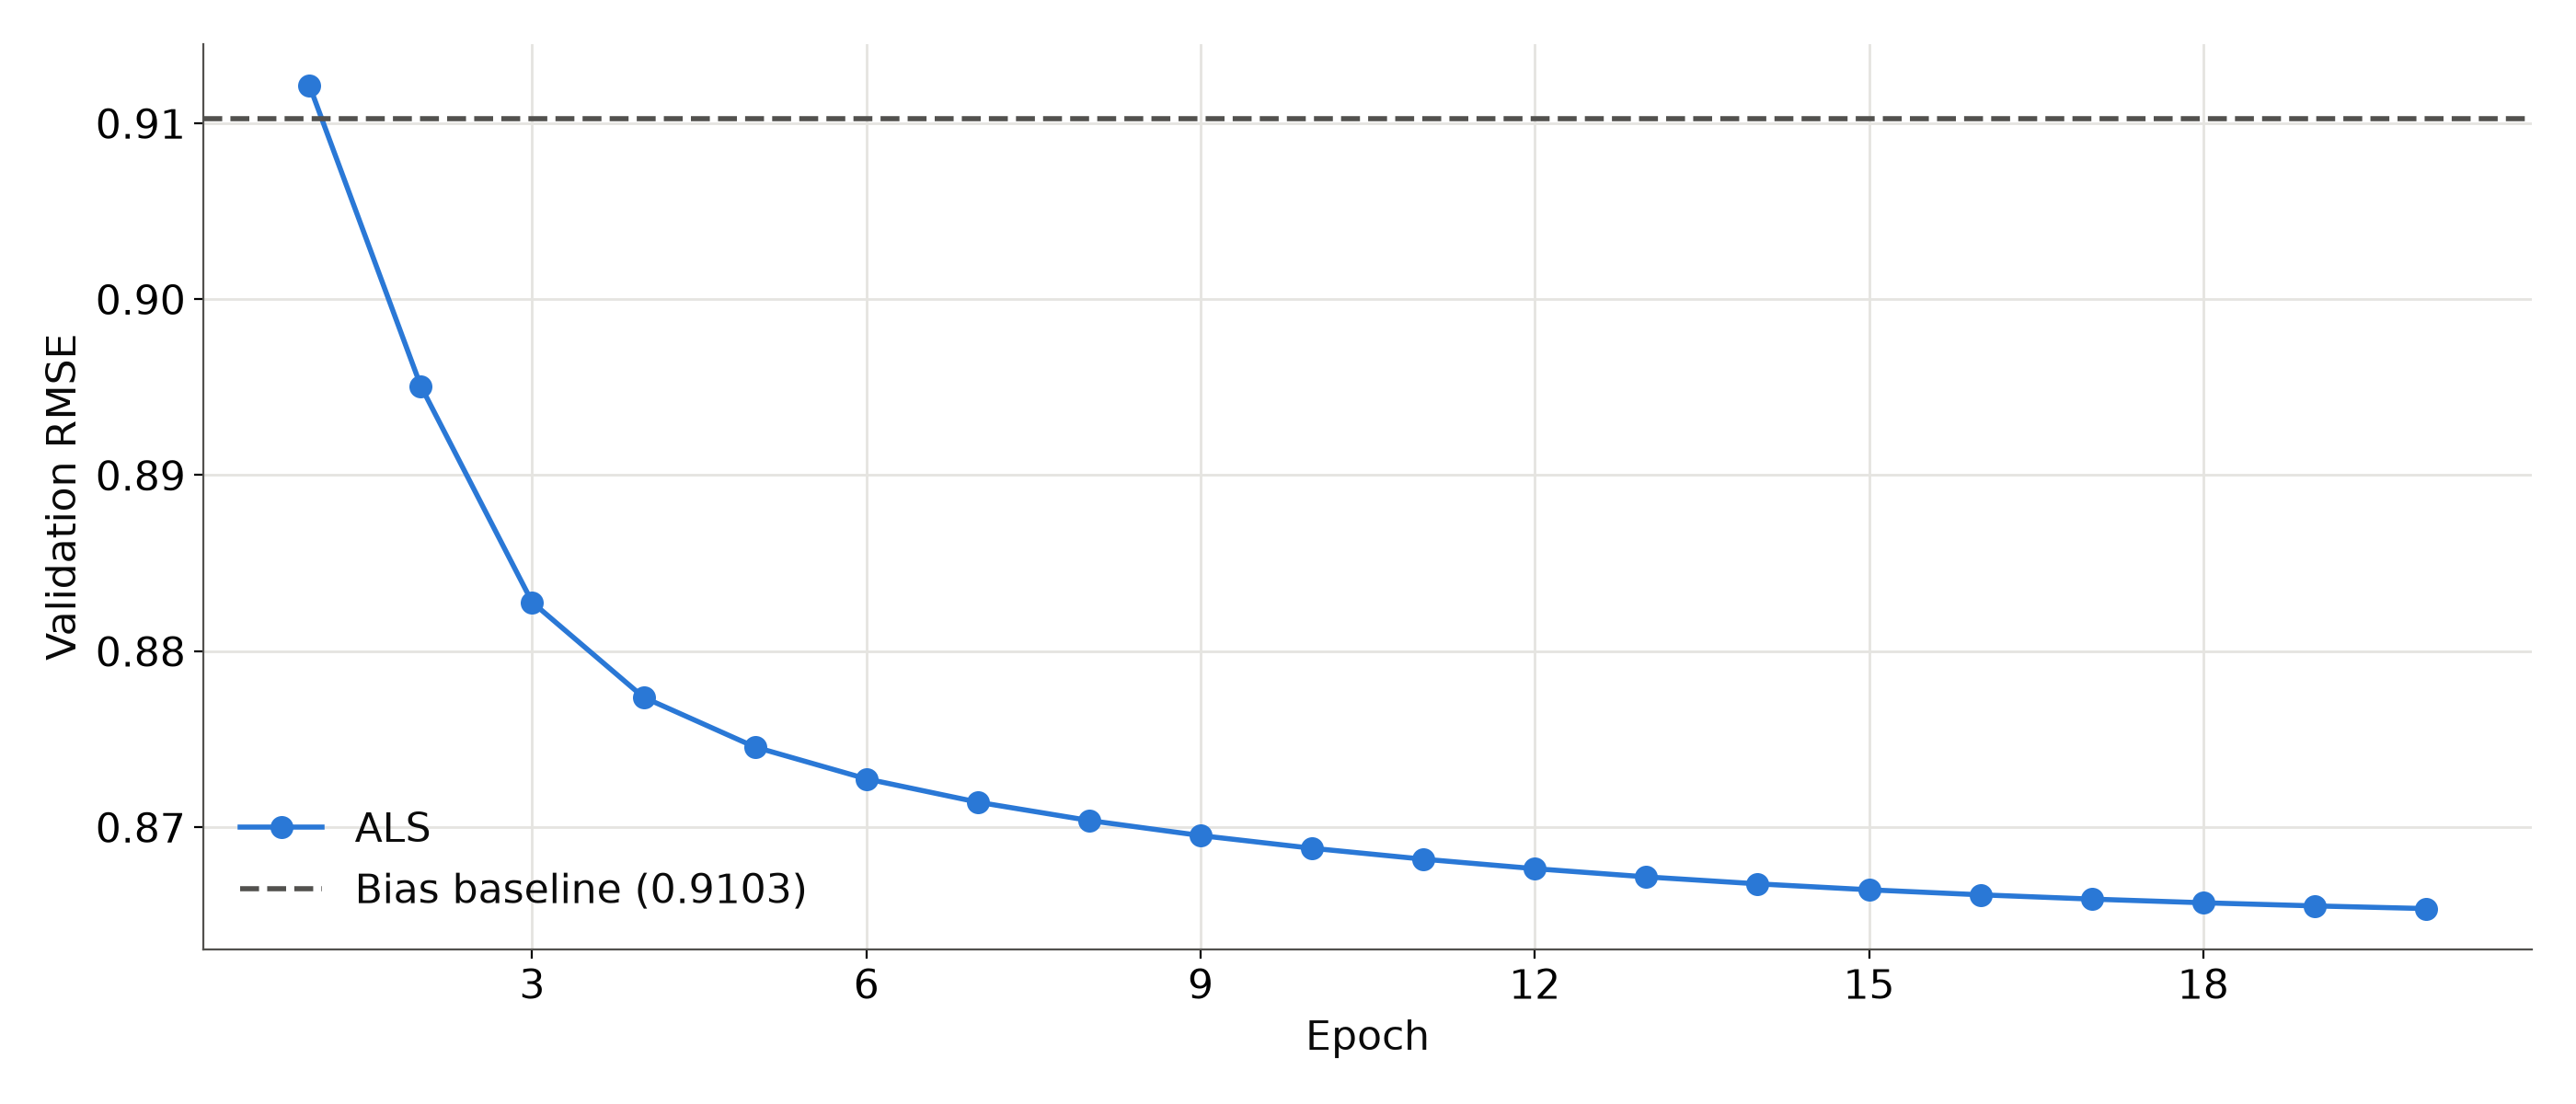
\includegraphics[width=0.85\linewidth]{figures/als_val_rmse_by_epoch.png}
  \caption{RMSE trên tập val theo vòng lặp; đường đứt nét là baseline.}
  \label{fig:als-convergence}
\end{figure}

Nhận xét:
\begin{itemize}
  \item ALS giảm RMSE val từ 0,9103 xuống 0,8654. Vòng đầu còn kém baseline (0,9121) vì $Q$ khởi tạo
        ngẫu nhiên; từ vòng 2 ALS đã tốt hơn, và 5 vòng đầu mang lại khoảng 80\% mức cải thiện.
  \item $J$ giảm ở mọi vòng, đúng như lý thuyết của bước nghiệm đúng. RMSE val ở vòng 20 vẫn còn giảm
        chậm, nên 20 vòng chưa phải điểm dừng tối ưu.
  \item RMSE train (0,728) thấp hơn khá nhiều so với RMSE val (0,865): mô hình đã khớp train tốt hơn
        dữ liệu mới, nên cần chọn $k$ và $\lambda$ trên tập val.
\end{itemize}

\subsubsection{Ví dụ thực tế: gợi ý cho hai người xem}

\paragraph{Người dùng có ID 1 (43 điểm trong train).}
Các phim người này chấm 5 điểm gồm \emph{Toy Story}, \emph{Beauty and the Beast}, \emph{Dumbo},
\emph{Mary Poppins}, \emph{Apollo 13} và \emph{Schindler's List}: chủ yếu phim gia đình, hoạt hình và phim
kinh điển. Bias $b_u = +0{,}25$ cho biết người này chấm dễ hơn mức chung. Năm phim ALS gợi ý là
\emph{The Shawshank Redemption} (4,90), \emph{Forrest Gump} (4,79), \emph{Rear Window} (4,75),
\emph{Seven Samurai} (4,74) và \emph{The Godfather} (4,72).

Điểm đáng chú ý là \emph{Forrest Gump}: baseline chỉ dự đoán 4,31, nhưng ALS cộng thêm $+0{,}48$ nhờ
$p_u^\top q_i$, đẩy phim này lên vị trí thứ hai. Đây đúng là phần cá nhân hóa mà baseline không có: một
phim nhẹ nhàng, cảm động, hợp gu người xem này. Các phim còn lại đều có $b_i$ cao (phim được đánh giá
cao chung), cho thấy gợi ý vẫn nghiêng về phim nổi tiếng.

Trên tập val của người này, ALS không phải lúc nào cũng đúng hơn. Với \emph{Pocahontas} (điểm thật 5),
baseline đoán 3,20 còn ALS đoán 3,39, gần hơn nhưng vẫn thấp; với \emph{Driving Miss Daisy} (điểm thật 4),
baseline đoán 4,12 còn ALS đoán 4,36, xa hơn. RMSE là trung bình trên hàng trăm nghìn điểm như vậy.

\paragraph{Người dùng có ID 3633 (10 điểm, ít nhất trong train).}
Với người có ít dữ liệu, vector $p_u$ được ước lượng từ rất ít phương trình nên dao động mạnh. Với
\emph{Star Wars: Episode IV} (điểm thật 4), baseline đoán 4,62 còn ALS đoán 3,99, gần như chính xác.
Nhưng với \emph{Star Wars: Episode I} (điểm thật 4), ALS đoán 2,79, tệ hơn baseline (3,55). Đây là minh họa
cho vấn đề \emph{khởi đầu lạnh} (cold start): dữ liệu càng ít, cá nhân hóa càng thiếu tin cậy, và $\lambda$
là thứ giữ cho dự đoán không đi quá xa baseline.

\subsubsection{Khả năng mở rộng}

Cùng code và cùng tham số được chạy thêm trên MovieLens-32M (Bảng~\ref{tab:als-scale}). Số điểm train tăng
khoảng 32 lần, thời gian tăng khoảng 49 lần, tức chi phí vẫn tăng cùng bậc với số điểm. Hai bộ dữ
liệu có thang điểm và tập người dùng khác nhau, nên không so sánh trực tiếp RMSE giữa chúng.

\begin{table}[H]
  \centering
  \caption{ALS trên hai bộ dữ liệu, $k = 20$, $\lambda = 10$, 20 vòng.}
  \label{tab:als-scale}
  \begin{tabular}{lrr}
    \hline
    Chỉ số & MovieLens-1M & MovieLens-32M \\
    \hline
    Số điểm train & $800\,203$ & $25\,604\,944$ \\
    Số hệ mỗi vòng & $9\,746$ & $285\,380$ \\
    Thời gian huấn luyện (s) & 1{,}45 & 71{,}6 \\
    RMSE val của baseline & 0{,}9103 & 0{,}8574 \\
    RMSE val của ALS & 0{,}8654 & 0{,}7769 \\
    \hline
  \end{tabular}
\end{table}

Phần tốn kém nhất mỗi vòng là dựng $Q_u^\top Q_u$, chiếm khoảng 84\% số phép tính với $k = 20$, chứ không
phải bước Cholesky. Vì vậy, với $k$ nhỏ, thời gian chủ yếu tăng theo số điểm; số hạng $k^3$ của Cholesky
chỉ đáng kể khi $k$ lớn.

\subsection{Kết luận}

\paragraph{Về phương pháp số.}
ALS cho thấy cách biến một bài toán tối ưu không lồi thành chuỗi bài toán tuyến tính quen thuộc: mỗi bước
là hàng nghìn hệ Ridge nhỏ (Chương 3), giải bằng Cholesky (Chương 2) trên dữ liệu lưu dạng CSR. Tham số
$\lambda$ vừa là công cụ thống kê chống học thuộc, vừa là công cụ số học: nó làm hệ của người ít dữ liệu
từ suy biến trở thành có nghiệm duy nhất, và giữ số điều kiện ở mức chỉ mất chưa tới 1 chữ số đáng tin
(Chương 1).

\paragraph{Về ý nghĩa cho hệ gợi ý.}
\begin{itemize}
  \item \textbf{Độ chính xác.} So với baseline, ALS giảm sai số trung bình khoảng 4,9\%. So với việc
        đoán mọi phim bằng điểm trung bình, mức giảm là khoảng 22\%. Phần cải thiện này đến từ cá nhân
        hóa: mô hình đưa những phim hợp gu riêng của từng người lên cao hơn danh sách ``phim được khen
        nhiều'' chung.
  \item \textbf{Chi phí vận hành.} Huấn luyện mất khoảng 1,5 giây trên ML-1M và khoảng 1 phút trên 32
        triệu điểm, trên một máy tính cá nhân. Ở quy mô này, có thể huấn luyện lại mỗi ngày khi có
        đánh giá mới; vì các hệ độc lập, có thể chia ra nhiều máy khi dữ liệu lớn hơn nữa.
  \item \textbf{Dễ vận hành.} Không có learning rate và $J$ luôn giảm, nên ít phải canh chỉnh hơn SGD.
\end{itemize}

\paragraph{Hạn chế và hướng tiếp theo.}
\begin{itemize}
  \item $k$ và $\lambda$ chưa được tinh chỉnh; cần dò lưới trên tập val trước khi so sánh trên tập test.
  \item Người dùng ít dữ liệu vẫn được dự đoán kém tin cậy (khởi đầu lạnh); có thể bổ sung thông tin như
        thể loại phim hoặc thông tin người dùng.
  \item Gợi ý còn nghiêng về phim nổi tiếng; nếu muốn đa dạng hơn cần thêm bước xếp hạng lại.
  \item Mô hình chỉ dùng điểm chấm tường minh, chưa dùng tín hiệu ngầm như việc người dùng đã xem phim
        nào; ALS có biến thể cho dữ liệu ngầm, có thể là hướng mở rộng.
\end{itemize}
